\documentclass[10pt,twocolumn]{article}
\newcommand{\PaperShortTitle}{ContextRuntime}
\usepackage{../paperstyle}
\usepackage{tikz}
\usetikzlibrary{arrows.meta,positioning,fit}
\hypersetup{
  pdftitle={ContextRuntime: Cache-Aware Admission and Lifetime Control for Token-Efficient Coding Agents},
  pdfauthor={Ankit Chauhan},
  pdfsubject={A cache-aware runtime for LLM coding-agent context optimization},
  pdfkeywords={LLM agents, token efficiency, context optimization, prompt caching, coding agents}
}

\title{\vspace{-1.2em}\textbf{ContextRuntime:}\\
\Large Cache-Aware Admission and Lifetime Control for Token-Efficient Coding Agents}
\author{Ankit Chauhan\\\small InfyU Labs}
\date{}

\begin{document}
\maketitle
\thispagestyle{fancy}

\begin{abstract}
Long-horizon coding agents repeatedly re-send a growing context.  Removing history can reduce
context workload but may invalidate a discounted prompt cache and create a more expensive rewrite;
loading all tool schemas up front can impose the same overhead on every call.  We present
ContextRuntime, a gateway that combines (i) pre-request admission control for unused tool schemas,
(ii) forward-only retirement of superseded or cold tool results, (iii) bounded retention of prior
thinking blocks, (iv) persistent mutation, and (v) a cache-aligned scheduler that fires only at a cold
boundary or when expected future cache-read savings exceed the suffix rewrite cost.  The gateway is
off by default, supports observe-before-enforce deployment, and fails open to the original request.
We evaluate the system in three evidence stages.  B6 is a preregistered live A/B with 24 graded
Django coding sessions: the integrated stack reduces pooled cumulative input by 41.5\% (14.87M to
8.70M tokens; four-task cluster-bootstrap 95\% interval 31.1--54.8\%) and passes a frozen operational
quality rule with 9/12 versus 10/12 successes.  However, unaligned history edits increase cache writes
68.1\%, leaving only 2.5\% lower CLI cost.  B7 fits a message-extent cache model that is exact on
11/12 native sessions and has 7.3\% median creation error on mutated sessions.  Replay says the
aligned policy correctly holds on short, cache-hot sessions and models a 61.5\% pooled dollar
reduction in 36 calibrated giant interactive sessions, with zero median-session gain; this tail result
is not live.  B8 then preregisters a live prediction on three pairs of chained three-task sessions.
Observed list-price cost falls 29.34\%, within 0.16 percentage points of the frozen 29.5\% prediction;
CLI cost falls 29.22\%, and quality is 9/9 in both arms.  Crucially, the scheduler makes no profitable
mid-session mutation: the B8 saving is essentially all admission.  The results show that context
optimization requires separate claims for workload, dollars, and task quality, and that cache-aware
inaction is a first-class systems behavior.
\end{abstract}

\section{Introduction}

An agent that calls a language model 50 times does not pay for an early tool schema or file read once.
The object remains in the request prefix and is processed on later calls, often as a discounted cache
read.  This creates two optimization opportunities and one trap.  Admission control can prevent a
large fixed object from entering at all.  Lifetime control can replace an obsolete object after it has
served its purpose.  But a lifetime edit changes the byte prefix, potentially converting cheap cached
input into an expensive cache write.  With the one-hour cache tier used by the evaluated client,
reads cost $0.1\times$ base input and writes $2\times$ \cite{anthropicPromptCaching}.  Deleting context
at the wrong time can lower token residency and increase dollar cost.

Prior work attacks important pieces of this problem.  LLMLingua-family methods compress supplied
prompts \cite{jiang2023llmlingua,jiang2024longllmlingua,pan2024llmlingua2}; MemGPT and recent coding
agents manage or compact memory \cite{packer2023memgpt,liu2026cat,verma2026focus,
zhang2026autocompact}; tool retrievers avoid exposing a large catalog
\cite{chen2024reinvoke,fei2025mcpzero}; and serving systems reuse KV state
\cite{kwon2023pagedattention,zheng2024sglang,gim2024promptcache}.  Recent API-level studies directly
measure prompt-cache strategy \cite{lumer2026cache,song2026capc,khailo2026keepalive}.  ContextRuntime
occupies the client-side systems boundary between these areas: it does not train a compressor or
control provider memory.  It decides what request content to admit, what prior content can be
replaced, and when a replacement is worth its cache consequence.

The design emerged from a measured elimination process, not a chosen final architecture.  Search
output compression was safe but too small in the whole-session denominator.  A semantic code-reading
surface received zero voluntary use in 11 runs.  Graph retrieval did not clear a joint recall--budget
gate.  An offline discovery call-collapse oracle looked promising, yet its forced eager implementation
raised live pooled input 55.6\%.  Those failures moved the system toward two mechanisms with large,
prospective surfaces: shrink the fixed prefix before turn one and control the lifetime of already
admitted objects.  The companion measurement paper details this evidence lineage.

This paper contributes:

\begin{enumerate}
  \item A deployable gateway that separates a forward-only safety planner from environment-specific
  history mutation, with observation, enforcement, persistence, recovery handles, and fail-open
  behavior.
  \item A cache-aligned scheduling rule that compares future read savings with the cost of rewriting
  the divergent suffix, rather than mutating at a fixed token or turn threshold.
  \item A message-extent cache simulator calibrated against live partial-prefix hits and an explicit
  price profile, used only for modeled claims unless a live preregistered test follows.
  \item A staged evaluation: 24 live graded B6 sessions, 66-session B7 replay, and a clean B8 live
  validation whose cost prediction misses by only 0.16 percentage points.
  \item An honest decomposition: B6 demonstrates context-workload reduction; B8 demonstrates live
  dollar reduction from admission and no-harm holding; the roughly 60\% giant-session lifetime payoff
  remains modeled.
\end{enumerate}

The artifacts and executable runtime are public \cite{contextruntime2026}.  Results come from one
client/provider configuration and Django tasks, so we treat them as design-partner evidence requiring
independent replication.

\section{Related Work}

\subsection{Prompt compression and context management}

Prompt compression removes low-information text or learns a compact representation.  LLMLingua
reports up to $20\times$ compression; LongLLMLingua is query-aware and targets position bias;
LLMLingua-2 trains a task-agnostic token classifier \cite{jiang2023llmlingua,
jiang2024longllmlingua,pan2024llmlingua2}.  RECOMP compresses retrieved evidence and can suppress
irrelevant augmentation, while ICAE and gist tokens learn latent summaries
\cite{xu2024recomp,ge2024icae,mu2023gist}.  These methods are plausible operators inside a runtime,
but a per-prompt ratio does not decide which agent objects to target or whether a query-dependent
rewrite destroys a discounted prefix.

Agent-memory work supplies the semantic control plane.  MemGPT uses virtual-memory tiers
\cite{packer2023memgpt}.  CAT makes context maintenance a callable tool and reports strong
SWE-bench-Verified accuracy under a bounded workspace \cite{liu2026cat}; Focus gives the agent
explicit checkpoint/consolidate operations and reports 22.7\% fewer tokens on five instances at
unchanged 3/5 success \cite{verma2026focus}; AutoCompact learns a compaction policy
\cite{zhang2026autocompact}.  ContextRuntime differs in four respects: retirement can be driven by
forward mechanical rules, exact payloads remain recoverable, scheduling includes provider cache
economics, and failure handling preserves the original request.  The approaches are complementary:
learned summaries can become another mutation type governed by the same cache gate.

\subsection{Tool admission and coding-agent interfaces}

Large tool catalogs create a fixed-prefix tax.  Re-Invoke, ToolRerank, and MCP-Zero retrieve a small
candidate set instead of presenting every schema \cite{chen2024reinvoke,zheng2024toolrerank,
fei2025mcpzero}.  Provider tool search similarly loads definitions on demand and reports large
reductions in initial tool context \cite{anthropicAdvancedTools,anthropicToolContext}.  Our admission
filter is simpler---it disallows schemas known unused for the evaluated headless task family---but it
is measured end to end and exposes a deployment interaction: Claude Code normally defers MCP tools,
yet falls back to eager loading when \texttt{ANTHROPIC\_BASE\_URL} targets a non-first-party proxy
unless tool search is explicitly configured \cite{anthropicMCP}.

Coding-agent research shows why task evaluation cannot be replaced by token metrics.  SWE-bench uses
real repository issues and objective tests \cite{jimenez2024swebench}.  SWE-agent demonstrates that
the agent-computer interface changes success \cite{yang2024sweagent}; Agentless obtains strong results
with a simpler localization--repair--validation pipeline \cite{xia2025agentless}; RepoCoder,
GraphCoder, and LocAgent improve repository context selection
\cite{zhang2023repocoder,liu2024graphcoder,chen2025locagent}.  ContextRuntime holds the agent's tool
surface and grading protocol constant between arms so that an efficiency intervention must retain
issue-resolution quality.

\subsection{KV caching and API economics}

vLLM/PagedAttention, SGLang/RadixAttention, Prompt Cache, ChunkAttention, RAGCache, CacheBlend, Preble,
and Parrot optimize memory placement, prefix sharing, prefill, or application-aware scheduling inside
an inference service \cite{kwon2023pagedattention,zheng2024sglang,gim2024promptcache,
ye2024chunkattention,jin2024ragcache,yao2025cacheblend,srivatsa2024preble,lin2024parrot}.  A proprietary
API client cannot move KV pages; it can observe usage fields and preserve or change request bytes.

The closest concurrent work studies this boundary directly.  Don't Break the Cache compares cache
strategies across three providers and more than 500 research-agent sessions
\cite{lumer2026cache}.  CAPC combines query-agnostic compression with explicit cache control and a
two-tier cost model \cite{song2026capc}.  Keepalive economics analyzes whether paying to refresh a
prefix across idle gaps is rational \cite{khailo2026keepalive}.  ContextRuntime adds coding-agent
object lineage, mutation/recovery safety, partial interior-hit calibration, and a live sequence that
separates admission from lifetime payoff.

\section{System Design}

\subsection{Goals and non-goals}

The gateway follows six requirements.

\begin{enumerate}
  \item \textbf{Preserve task semantics.}  Exact edit preconditions and the most recent object for a
  warm key remain; a retired payload is replaced by a recovery handle.
  \item \textbf{Use only forward information.}  Production decisions cannot use the future labels
  available to an offline oracle.
  \item \textbf{Separate safety from timing.}  The planner decides \emph{what} is eligible; the cache
  scheduler decides \emph{when} to expose a new byte divergence.
  \item \textbf{Keep the mutated stream stable.}  Once a mutation fires, it is reapplied to every
  subsequent request so history does not snap back.
  \item \textbf{Fail open.}  Parsing, logging, or upstream rejection must not block the agent; the
  unmodified body is the recovery path.
  \item \textbf{Expose evidence grades.}  Live, modeled, and counterfactual results remain distinct.
\end{enumerate}

We do not train a semantic compressor, change the model, promise cross-provider cache equivalence, or
claim that discarded content is universally irrelevant.  The runtime is a policy and accounting layer.

\begin{figure*}[t]
\centering
\begin{tikzpicture}[
  node distance=0.45cm and 0.48cm,
  box/.style={draw=CRBlue,rounded corners=2pt,fill=CRPale,minimum height=0.72cm,text width=2.55cm,align=center,font=\small},
  sub/.style={draw=CRMuted,rounded corners=2pt,fill=white,minimum height=0.62cm,text width=2.35cm,align=center,font=\footnotesize},
  arrow/.style={-{Latex[length=2mm]},thick,color=CRMuted}
]
\node[box] (client) {Coding-agent client\\full request};
\node[box,right=of client] (admit) {Admission control\\remove/defer schemas};
\node[box,right=of admit] (gateway) {Context gateway\\observe or enforce};
\node[box,right=of gateway] (provider) {Model API\\usage + cache state};
\draw[arrow] (client) -- (admit);
\draw[arrow] (admit) -- (gateway);
\draw[arrow] (gateway) -- (provider);
\draw[arrow] (provider.south) to[bend left=18] node[below,font=\footnotesize,color=CRMuted]{response / fallback signal} (gateway.south);

\node[sub,below=0.65cm of gateway,xshift=-2.55cm] (planner) {Safety planner\\superseded + cold tail};
\node[sub,right=of planner] (scheduler) {Cache scheduler\\cold or break-even};
\node[sub,right=of scheduler] (mutator) {Persistent mutator\\stub + recovery ref};
\draw[arrow] (planner) -- (scheduler);
\draw[arrow] (scheduler) -- (mutator);
\draw[arrow] (gateway) -- (scheduler);
\draw[arrow] (mutator.north) to[bend right=18] (gateway.south);
\end{tikzpicture}
\caption{ContextRuntime request path.  Admission changes the first request and remains prefix-stable.
The gateway reconstructs objects, asks the forward planner what is eligible, asks the scheduler
whether a new cache divergence pays, and applies the fired set persistently.  Observation mode logs
the same decision without mutation; all exception paths preserve the original request.}
\label{fig:architecture}
\end{figure*}

\subsection{Admission control}

Tool schemas are unusually leveraged because they are fixed, early, and often unused.  The evaluated
admission profile uses the client's \texttt{--disallowedTools} mechanism to remove definitions that
never appeared in the headless task traces.  A zero-model-call capture reduced the transmitted tool
set from 82 schemas (46.1k cl100k-estimated tokens) to six (5.6k).  The filter is configured outside
the model and therefore does not require voluntary tool-search adoption.

Admission is conservative.  The six retained tools provide repository reading, search, editing, and
execution needed by the task harness.  The system never silently removes a schema selected by the
active profile.  Other deployments should derive their own allowlist from observe-mode traces; the
particular 82-to-6 profile is not a universal recommendation.

\subsection{Forward retirement planner}

The planner observes tool-result objects in call order.  Each object has an identifier, admission
turn, estimated token size, a supersession key such as \texttt{path:module.py} or a command signature,
and an optional recovery reference.  A later object with the same key makes earlier objects
mechanically \emph{superseded}.  The most recent object for a key is retained while the key is warm.
If a key has not been touched for $L=5$ turns, its older object becomes a \emph{cold-tail} candidate.
Plans are normally batched at $K=10$ turns to amortize rewrites.

The mutator replaces an eligible \texttt{tool\_result} with a small explicit stub, not an invented
summary.  The stub names a content-addressed handle or instructs the agent to rerun/re-read the source.
The planner is pure and environment-independent.  A subscription client that cannot rewrite history
uses an unsupported mutator; a gateway or custom loop that owns the message array uses the in-process
mutator.  This seam prevents an offline policy from being confused with a deployable mechanism.

\subsection{Thinking lifetime}

Models can retain prior thinking or redacted-thinking blocks in later requests.  A keep-$N$ rule
removes those blocks from all but the most recent $N$ assistant messages; the experiments use
$N=1$.  Thinking removal is tracked separately because displayed transcript text can omit the
payload while provider usage still reflects it.  Under cache alignment, a thinking frontier advances
only when a mutation fires, making the edited byte stream stable between fires.

\subsection{Cache-aligned scheduler}

Let $G$ be the tokens in new pending retirements, $S$ the estimated suffix tokens that would need to
be recreated after the earliest edit point, $E$ the expected remaining calls, $r$ the cache-read price,
and $w$ the cache-write price.  A mutation clears the break-even gate when
\begin{equation}
rGE \ge (w-r)S. \label{eq:breakeven}
\end{equation}
The default evaluated profile uses $r=0.1$, $w=2.0$, and $E=8$.  If each retired token requires one
suffix token to be rewritten, a write requires 19 future reads to break even.  Equation
\ref{eq:breakeven} can still fire with $E<19$ when one early divergence retires substantially more
pending content than the suffix it rewrites.

The scheduler has three modes: \texttt{off}, \texttt{cold}, and \texttt{gated}; the default is off.
Cold starts are safe moments to establish the mutated stream.  A TTL-gap rule can also fire when the
cache is believed expired, although B8 v1 reveals that nominal TTL is soft at 65 minutes; deployments
should prefer observed miss telemetry or a conservative margin.  Gated mode adds Equation
\ref{eq:breakeven}.  The scheduler decides timing only and cannot promote an unsafe object.

The key state invariant is persistence.  A fired identifier enters a set and is rewritten on every
later request.  Reapplication is byte-stable and does not create another divergence.  Only newly
eligible objects can cause a new cache invalidation.  This repairs the B6 ``flash'' behavior, in which
retirement applied only on batch-boundary requests and history returned on intervening calls.

\subsection{Operational safety}

Modes form an escalation path: off passes through, observe logs opportunities, and enforce mutates.
Unexpected parsing errors return the untouched request.  The live harness also retries an original
body if an upstream response rejects a mutated request.  Logs record the eligible count, tokens,
boundary, fired reason, gap, pending mass, suffix estimate, persistent reapplications, applied
retirements, stripped thinking, and fallback count.  These fields turn ``no harm'' from an assumption
into a measurable endpoint.

\section{Evaluation Method}

\subsection{Research questions}

\begin{description}
  \item[RQ1:] Does integrated admission and lifetime control reduce cumulative live input while
  preserving objectively graded coding quality?
  \item[RQ2:] Can a calibrated cache model identify when lifetime mutation earns dollars and when it
  should hold?
  \item[RQ3:] Does a preregistered live experiment validate the model and the no-harm behavior of the
  aligned stack?
\end{description}

\subsection{B6: integrated live A/B}

B6 contains four modern Django SWE-bench-Verified instances, three interleaved paired repetitions,
and two arms, for 24 live sessions.  Every run uses the same Sonnet model, prompt, budget cap, and fresh
worktree.  The native arm is stock headless Claude Code.  The treatment arm applies 82-to-6 schema
admission plus gateway enforcement with lag-five/batch-ten retirement and thinking keep-one.  Graph,
discovery, and search-replacement mechanisms are excluded because earlier gates closed them.

The preregistered primary endpoint is
\begin{equation}
R=\frac{\sum_t P_{t,\mathrm{T}}}{\sum_t P_{t,\mathrm{N}}},\quad
P_t=R_t+W_t+U_t,
\end{equation}
reported per task and pooled.  API calls are reconstructed by merging transcript records with the same
\texttt{requestId}; sidechains are excluded.  A run succeeds only when official FAIL\_TO\_PASS tests
pass and PASS\_TO\_PASS tests remain green.  The frozen operational quality rule requires total
treatment successes to be at least native successes minus one, with no task at 0/3 treatment when
native is 3/3.  This is a program decision rule, not a statistically powered non-inferiority trial.

No session times out or reaches the budget cap.  We add a post-hoc task-cluster bootstrap interval for
effect-scale uncertainty; four tasks make it intentionally coarse, and the preregistered pooled ratio
remains the decision endpoint.

\subsection{B7: calibrated replay}

B7 simulates cached prefix extents with TTLs and partial interior hits.  On append-only call $t$, the
largest alive matching extent is read and the remaining suffix is created.  When history first differs
at depth $c$, the request may read the largest matching prefix before $c$; stale longer extents are
discarded and the new full extent is stored.  Inputs are observed per-call API token totals, so text
token estimation is not on the pricing critical path.

Calibration uses the 12 B6 native timelines and the 12 observed B6 mutation schedules.  A second
replay covers 54 real interactive sessions, up to 2,315 calls and $1.2$ billion cumulative input
tokens.  Because sessions with native compaction violate the simple append-only model, results are
reported for all 54 and for a frozen well-calibrated subset of 36 with absolute cache-creation error
at most 20\%.  Policies are native, persistent-but-unaligned, cold-only, gated, and an oracle using the
true remaining-call count.

We price calls in base-input-token equivalents (BITE):
\begin{equation}
\mathrm{BITE}=0.1R+2.0W+1.0U+5.0O.
\end{equation}
Percentage deltas are more portable than absolute dollars because the interactive archive mixes
models.

\subsection{B8: preregistered live validation}

B8 v2 contains three live pairs.  Each session chains three graded Django tasks in one conversation,
with a 60-second pause between tasks.  The native arm is unchanged.  The treatment combines admission
with the persistent gated gateway.  Before the first paid v2 run, the B7 machinery predicts a 29.5\%
pooled BITE reduction and freezes a validation band of 22--36\% reduction.  The primary endpoint is
pooled BITE; secondary endpoints include CLI-reported cost, cumulative input, fires by reason,
fallbacks, and nine task grades per arm.

An earlier v1 experiment is preserved as a confounded negative result.  Its treatment used a custom
base URL without admission and 65-minute gaps.  The proxy caused the client to eagerly include tool
schemas, and the nominal one-hour TTL remained warm.  Per preregistration, post-hoc correction does not
rescue v1; the findings instead determine the clean v2 design.

\begin{figure*}[t]
\centering
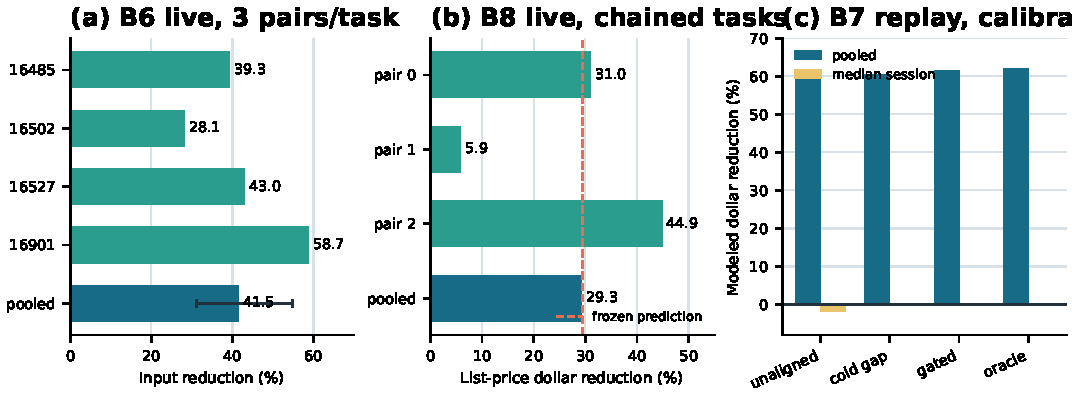
\includegraphics[width=\textwidth]{../figures/runtime_results.pdf}
\caption{Three evidence stages.  (a) B6 live cumulative-input reduction by task and pooled; the pooled
whisker is a post-hoc four-task cluster-bootstrap 95\% interval.  (b) B8 v2 live BITE reduction by pair
and pooled; dashed line is the frozen prediction.  (c) B7 modeled dollar reduction on 36
well-calibrated interactive sessions.  The pooled/median split shows that the modeled lifetime value is
tail-concentrated.  B7 values are not live savings.}
\label{fig:results}
\end{figure*}

\section{B6: Live Workload Reduction}

\begin{table*}[t]
\centering
\caption{B6 preregistered primary endpoint and objective success counts.  Input is the sum of cache
read, cache creation, and uncached input over three runs per arm.}
\label{tab:b6}
\small
\begin{tabular}{lrrrr}
\toprule
Task & Native input & Treatment input & Reduction & Success N/T \\
\midrule
16485 & 2,772,225 & 1,682,341 & 39.3\% & 3/3 \\
16502 & 4,753,322 & 3,418,567 & 28.1\% & 2/0 \\
16527 & 3,606,230 & 2,055,051 & 43.0\% & 3/3 \\
16901 & 3,734,336 & 1,543,827 & 58.7\% & 2/3 \\
\midrule
Pooled & 14,866,113 & 8,699,786 & 41.5\% & 10/9 \\
\bottomrule
\end{tabular}

\end{table*}

Table~\ref{tab:b6} shows the primary result.  Pooled cumulative input falls from 14,866,113 to
8,699,786 tokens, $R=0.5852$, a 41.5\% reduction.  All four task-level pooled effects are positive,
ranging from 28.1\% to 58.7\%.  Ten of 12 individual pairs reduce input; stochastic trajectory length
produces two reversals and a wide pair range.  The post-hoc task-cluster bootstrap 95\% interval is
31.1--54.8\%.  With only four clusters, this interval is a sensitivity summary rather than a basis for
population generalization.

Objective quality is 10/12 native and 9/12 treatment, passing the frozen rule exactly at its bound.
Task 16502 is the residual risk: treatment is 0/3 while native is 2/3.  All four failures across arms
share the same shallow-fix mode; one native and one treatment patch are essentially the same.  The
sample cannot rule out a treatment effect, and we do not use the cross-arm similarity to erase the
failure.  Task 16901 moves in the other direction, with treatment 3/3 and native 2/3.

Mechanism health is clean: 353 tool results are retired, 1,794 thinking blocks are stripped, and no
mutated request falls back.  Same-path repeat reads are 11/36 native and 12/39 treatment, providing no
evidence of a retirement-induced reread tax.  All runs receive real FAIL\_TO\_PASS and
PASS\_TO\_PASS grading rather than process-success labels.

\claimbox{\textbf{RQ1 (\live):}  The integrated stack reduces cumulative input by 41.5\% and passes
the preregistered operational quality gate.  The result is a context-workload claim in four Django
tasks, not a universal token or quality estimate.}

\subsection{The dollar contradiction}

B6 also exposes why cumulative input and dollars must be separate.  Treatment makes 311 API calls
versus 279 (+11.5\%), lowers cache reads from 14,478,012 to 8,047,610 (44.4\%), increases cache
creation from 387,545 to 651,554 (68.1\%), and increases output from 85,274 to 93,677 (9.9\%).  CLI
cost moves only from \$7.98 to \$7.78, a 2.5\% reduction.  Repricing at the observed one-hour tier
reconstructs a 2.8\% reduction, nearly matching the CLI.

The cause is observable in the gateway schedule.  Retirement fires only on batch boundaries; the
full original history reappears between them.  Each boundary pays another suffix creation and the
retirement saving lasts one call.  Thinking removal and admission remain applied on every call and
carry most of the residency effect.  This ``flash'' mutation is the failure that B7 persistence and
cache alignment repair.

\section{B7: Cache Model and Scheduling}

\subsection{Calibration}

Three platform facts are learned rather than assumed.  First, the client requests the one-hour cache
tier, so the write multiplier is 2.0 rather than 1.25.  Second, the provider serves partial interior
hits: editing at depth $x$ preserves the matching prefix before $x$.  Third, back-to-back sessions can
begin with a warm shared fixed prefix.  Incorporating these facts makes the append-only simulator exact
on 11/12 B6 native sessions; the remaining session contains one retry anomaly among 279 native calls.
Replaying the 12 observed treatment mutation schedules yields about 1\% cache-read error and 7.3\%
median absolute cache-creation error.  On the 54 interactive sessions, median absolute creation error
is 3.0\% but p90 is 64\%, revealing a compaction-heavy regime outside the model.

\subsection{Two workload regimes}

On the 11 well-calibrated B6 native timelines, persistent unaligned mutation is modeled to increase
dollars 8.4\% while reducing residency 9.6\%.  Cold-only, gated, and oracle policies fire zero times
and change cost by zero.  Even an oracle finds no profitable mid-session edit in these short, hot
sessions.  Holding is the correct action.

On the 36 well-calibrated interactive sessions, the picture changes:

\begin{table}[h]
\centering
\caption{B7 cache-policy replay on the well-calibrated interactive subset.  All values are modeled.}
\label{tab:b7}
\small
\begin{tabular}{lrrrr}
\toprule
Policy & Pooled $\Delta\$$ & Median $\Delta\$$ & $\Delta$res. & Fires \\
\midrule
Unaligned & $-61.9\%$ & $+1.9\%$ & $-74.2\%$ & 807 \\
Cold gap & $-60.4\%$ & $0.0\%$ & $-65.4\%$ & 125 \\
Gated & $-61.5\%$ & $0.0\%$ & $-67.0\%$ & 2,514 \\
Oracle & $-62.1\%$ & $0.0\%$ & $-73.7\%$ & 4,287 \\
\bottomrule
\end{tabular}
\end{table}

The pooled result is dominated by giant sessions.  For gated scheduling, only 8/36 sessions have a
positive modeled saving and 28 are unchanged; the top five sessions contribute about 90.4\% of total
modeled savings.  The median session gains nothing.  Unaligned scheduling reduces pooled cost yet
regresses the median, exactly the behavior seen on B6-style timelines.  Gated scheduling comes within
0.6 percentage points of the oracle's pooled cost while avoiding negative modeled deltas.

\claimbox{\textbf{RQ2 (\modeled):}  One policy adapts across regimes: hold in short cache-hot sessions,
fire in the long tail when the read annuity dominates the rewrite.  The 61.5\% pooled interactive
payoff remains a replay result, not a live claim.}

\section{B8: Preregistered Live Validation}

\begin{table*}[t]
\centering
\caption{B8 v2 primary and secondary live effects.  Each pair contains three chained tasks per arm;
all 18 task instances pass objective grading.}
\label{tab:b8}
\small
\begin{tabular}{lrrrr}
\toprule
Pair & Native BITE & Treatment BITE & Dollar reduction & Residency reduction \\
\midrule
0 & 894,926 & 617,611 & 31.0\% & 43.5\% \\
1 & 551,222 & 518,781 & 5.9\% & 11.0\% \\
2 & 737,518 & 406,481 & 44.9\% & 55.9\% \\
\midrule
Pooled & 2,183,665 & 1,542,873 & 29.3\% & 40.1\% \\
\bottomrule
\end{tabular}

\end{table*}

Pooled BITE falls from 2,183,665 to 1,542,873, a 29.34\% reduction.  The frozen prediction is
29.5\%, so error is $-0.16$ percentage points and the result is inside the preregistered 22--36\%
validation band.  The independent CLI report falls from \$6.553 to \$4.638, or 29.22\%.  Cumulative
input falls 40.10\%, from 14,158,182 to 8,480,551.  Pair-level dollar reductions are 31.0\%, 5.9\%,
and 44.9\%; reporting all three makes the replication variance visible.  Quality is 9/9 in both arms.

No treatment request falls back.  Each gateway fires once at cold start.  The predicted marginal
break-even fires do not occur, and no tool result or thinking block is retired mid-session.  This is
not a failure hidden by the aggregate: it is the scheduler's desired no-harm behavior under one-hour
write pricing.  The live cost saving is essentially all schema admission.  The model predicts the
aggregate accurately because lifetime's expected contribution in this shape was already small, but
its individual fire-count forecast is wrong.

\claimbox{\textbf{RQ3 (\live):}  The admission-plus-gated stack cuts list-price cost 29.34\%, within
0.16 points of the frozen prediction, and CLI cost independently agrees.  The test validates admission
pricing and cache-aware holding; it does not validate the B7 giant-session firing payoff.}

\subsection{The confounded v1 is part of the result}

B8 v1 used a proxy without admission and 65-minute gaps.  Its treatment moved outside the frozen band
because setting a custom base URL disabled normal MCP tool-schema deferral.  The first treatment
request carried about 84,676 tokens versus 41,554 for native, followed by full-prefix rewrites as the
tool list changed.  One rewrite occurred when the gateway made no mutation, isolating the client
behavior from the scheduler.  Provider documentation now describes this fallback explicitly
\cite{anthropicMCP}.

Native requests also retained cache hits after 65 minutes.  Nominal TTL therefore did not identify a
free boundary.  Per the protocol, a post-hoc subtraction that would place one pair near the predicted
band is not counted as validation.  Instead, v1 yields two product rules: a proxy must preserve tool
deferral or perform admission itself, and a time threshold alone is not proof that a cache is cold.

\section{Discussion}

\subsection{The result is three claims, not one}

The experiments support three different statements.

\begin{enumerate}
  \item \textbf{Live workload:} admission plus unaligned lifetime control reduces cumulative input
  41.5\% in B6, with a frozen operational quality rule passed.
  \item \textbf{Live dollars:} admission plus gated holding reduces BITE 29.34\% and CLI cost 29.22\%
  in B8; the realized saving is admission.
  \item \textbf{Modeled lifetime dollars:} gated retirement reduces pooled cost about 61.5\% in a
  calibrated replay of giant sessions, but the median is zero and no live firing-regime A/B exists.
\end{enumerate}

Combining the largest percentages would be invalid.  They refer to different workloads, policies, and
evidence grades.  The honest current product story is simpler: audit and shrink the fixed prefix
first; observe cache behavior; enable persistent lifetime mutation only when Equation
\ref{eq:breakeven} clears; retain the original request as a safety path.

\subsection{Why inaction is an optimization}

Efficiency systems are often evaluated by how often they transform input.  ContextRuntime's key
behavior is sometimes to do nothing.  On a hot prefix, each deleted token saves $r$ on a future read
but can force $w-r$ of new creation in the divergent suffix.  With $w-r=1.9$ and a conservative
remaining-call estimate, most ordinary sessions cannot amortize the edit.  A fixed threshold would
mutate precisely when the cache makes mutation least attractive.  Gated holding is therefore a
positive result with a measurable counterfactual: it removes B6's modeled +8.4\% cost regression and
adds zero overhead to B8 beyond admission.

\subsection{Provider portability}

The runtime parameterizes TTL, read, write, and output multipliers.  Under free or cheap cache writes,
Equation~\ref{eq:breakeven} fires much more often; under expensive long-TTL writes it holds.  The same
session artifacts can be repriced, but provider profiles other than Anthropic one-hour are currently
offline presets, not live validations.  Cache-key construction, minimum cacheable length, eviction,
and partial-hit semantics may differ, so portability requires a small calibration suite before
enforcement.

\subsection{Combining with learned compression}

The planner currently replaces exact old payloads with recovery stubs.  A learned compressor could
reduce $G$ earlier or preserve richer semantic state.  The scheduler remains useful: any generated
summary changes bytes and should be introduced when its expected read annuity clears the rewrite cost.
Conversely, cache-aware prompt compression such as CAPC \cite{song2026capc} could improve admission
while the retirement planner supplies object lifetime.  The architectural boundary supports these
compositions without treating a learned model as a safety proof.

\section{Limitations and Future Work}

\textbf{Scale and scope.}  B6 has four task clusters and B8 three session pairs, all Django and one
client/model family.  Large within-task variance is visible.  The operational quality gate is not a
powered statistical non-inferiority test.  Replication should expand repositories, languages,
models, and agents while preserving paired prompts and objective grading.

\textbf{The tail is not live.}  B7's roughly 60\% pooled payoff appears in a few giant interactive
sessions and is zero for the median.  A decisive next experiment must enter that firing regime under
controlled cost, preregister both pooled and distributional endpoints, and inspect recovery behavior.

\textbf{Cache observability.}  The scheduler infers state from timing and a calibrated extent model.
B8 v1 shows that nominal TTL is soft.  Provider-supplied cache identifiers or explicit hit telemetry
would make cold-boundary decisions more reliable.  Until then, TTL-gap firing should use conservative
margins or be disabled.

\textbf{Token estimation off the critical path.}  Observed API usage prices sessions exactly, but
pending retirement size and suffix depth use calibrated character/token estimators.  Estimation error
can change a knife-edge fire, as B8's predicted nine marginal fires versus zero observed illustrates.
A safety margin or online calibration should accompany provider transfer.

\textbf{Mutation semantics.}  Supersession is mechanically strong; cold-tail retirement is a policy
assumption with a recovery path.  Zero fallbacks across 17 live enforce sessions and no observed B6
reread tax are encouraging but do not prove semantic safety.  Future work should log recovery-handle
use, causal rereads, and failures over larger diverse workloads.

\textbf{Private interactive traces.}  The 54-session B7 archive is not redistributed.  Aggregate
replay output and source code are public, but independent replication requires new traces.  The live
B6/B8 aggregate artifacts and gateway decision logs are committed.

\section{Conclusion}

Context optimization in coding agents is not a single compression problem.  Fixed schemas, old tool
results, hidden reasoning, future turns, and provider cache state interact.  ContextRuntime separates
admission, safety, mutation, and timing so that each can be measured independently.  Live B6 results
show a 41.5\% cumulative-input reduction, but also reveal that unaligned edits turn cache reads into
writes and nearly erase dollar savings.  The calibrated B7 model turns this contradiction into a
break-even scheduler.  Live B8 then validates a 29.34\% cost reduction against a frozen 29.5\%
prediction while the scheduler correctly refuses unprofitable mid-session work.  Today, admission is
the demonstrated dollar lever; cache-aligned lifetime savings in giant sessions remain a precise,
testable hypothesis rather than a marketed result.

\section*{Artifact and Reproducibility Note}

\noindent\textbf{Code and artifacts:} \repo\par\smallskip
The repository contains the B6 and B8 protocols, task-level live artifacts, treatment decision logs,
B7 cache simulator, provider profiles, scheduler and gateway code, regression tests, and a script that
recomputes all tables and figures without model calls.  From the repository root, run
\texttt{python3 papers/scripts/generate\_assets.py}, then build this source with
\texttt{latexmk -pdf main.tex}.

\bibliographystyle{plain}
\bibliography{../references}

\end{document}
